%
% File TwitterBullying.tex
%

\documentclass[11pt,letterpaper]{article}
\usepackage{Formatting}
\usepackage{times}
\usepackage{latexsym}
\usepackage[square,comma,numbers,sort&compress]{natbib} % for numerical style references
\usepackage{tabularx}
\usepackage{graphicx}
\setlength\titlebox{6.5cm}    % Expanding the titlebox
\newcommand{\at}{\makeatletter @\makeatother}

\title{
Using Sentiment Analysis to Identify Bullying Using Twitter
%\Thanks{
%}
    }

\author{
	Michael Meding\\
  	University Massachusetts Lowell\\
	1 University Ave\\
	Lowell, MA 01854, USA\\
   {\tt mikeymeding@gmail.com}
	\And  
   Hoanh Nguyen\\
	University Massachusetts Lowell\\
	1 University Ave\\
	Lowell, MA 01854, USA\\
	{\tt soujiroboi@gmail.com }
}



\date{}

%  CRAP WE NEED TO INCLUDE
%   a. an abstract, describing briefly what you have done and results you obtained
%   b. an introduction, a statement of the problem you are trying to address and a brief description of your solution
%   c. related work section, describing relevant results from other people's efforts to solve this problem
%   d. description of your methodology, including 
%       - machine learning methods, 
%       - data sets used in the study,
%       - experimental setup and and evaluation methods;
%   f. description of your results.
%   g. discussion of results, conclusions of your study, future directions for this work

\begin{document}
\maketitle
\begin{abstract}
  Twitter is a social network where users can communicate publicly with short text statements called tweets. However, it should come as no surprise that not all of these tweets have good intention. With the rise of social media usage in youth, Twitter has gone from a calm social environment to connect with others to a hostile place. This program identifies users who have a high likelihood of being a bully through the use of sentiment analysis and machine learning. We did this by taking data from Twitter and analysing the aggressiveness of a tweets and hashtags using both the SentiWordNet database, Harvard Inquirer, and ArkTweetNLP. This data is then run through a Machine Learning algorithm to determine if a user can be classified as a bully based on the sentiment of the words used and based on previously seen tweets.
\end{abstract}

\section{Introduction}
%   b. an introduction, a statement of the problem you are trying to address and a brief description of your solution
\paragraph{}
What is bullying? Bullying is when a person is constantly being exposed to negative actions by another individual or group of individuals and can involve both physical and mental abuse. Some common forms of mental bullying include name calling, making threats, and spreading rumours. Since the creation of social media sites, bullying has become a problem outside of the school environment and is now considered a serious national health issue among adolescents~\cite{SentiBullying}. Bullies are using the internet as an outlet to post negative comments about someone, and unlike in a school environment, they rarely see backlash for what they post on social media sites.
\paragraph{}
This program identifies Twitter users who are bulling those around them. To accomplish this task, the program trains a binary classifier to decide if a single tweet is bullying or not. However, further research has shown that bullying cannot fully be defined by a simple binary "yes" or "no". Bullying, in a broad sense, can be classified into many different categories beyond that of just the bully and the victim. For example, when observing a bully in action on Twitter, you will notice that there are a lot of supporting users who do not have anything to do directly with a given bullying situation. This leads to a large amount of ambiguity when trying to decide whether someone is a bully, defender, victim, or accuser.
\paragraph{}
For a tweet to be cleanly identified by a computer as being bullying it must have both an aggressive statement and a subject or direction towards that anger. This would completes the simple bully to victim relation. One of the major flaws with this is that often times the subject of an aggressive tweet is implied, thus making it very difficult for a machine to identify a subject. Another problem is sarcasm. Computers cannot accurately identify sarcasm using only text and unfortunately bullies often use sarcasm. Our solution to this problem was to use an assisted machine learning algorithm. The data sets were manually annotated by a human who could only use the information contained within a given tweet to decide if that user is a bully or not. By using a brute force approach, we achieved a high accuracy when tweets directly mention a subject. Given the small data set, the annotated results were surprising.


\section{Related Work}
%   c. related work section, describing relevant results from other people's efforts to solve this problem
%   We probobly could have done more research before beginning but oh well.
%   I found a few related items and publications at the website below.
\paragraph{WSIC}
% http://research.cs.wisc.edu/bullying/publications.html
Two years ago, the University of Wisconsin completed a project on the study of bullying in Twitter that heralded lots of media coverage, including several articles from \textit{The Huffington Post} and \textit{Time Magazine}. The University of Wisconsin's code used a set of static words as search terms for tweets, then classified the tweets using a very small pre-existing bullying model. This model did yield some results but the efficacy left much to be desired. The first version of the University's code was made public and can easily be seen that it is quite primitive by comparison to our project. Unfortunately, the university didn’t release the data sets that they used for the projects so the reported results could not be confirmed.

\paragraph{Psychology}
% talk about bullying from a psycological perspective
% http://extension.fullerton.edu/professionaldevelopment/assets/pdf/bullying/sticks_and_stones.pdf
This project required looking at bullying through many different lenses. To be able to identify bullies you need to be able to understand them from a psychological standpoint. The paper \textit{Sticks and Stones Can Break My Bones, But How Can Pixels Hurt Me?} ~\cite{PixelsHurtMe} suggests that youth today have adopted a new type of bullying through social media. This new form of electronic communication makes it much easier for young users to say things that they would not normally say in person. Often times users will have a completely different persona online than in person.



\section{Methodology}
%   d. description of your methodology, including 
%       - machine learning methods, 
%       - data sets used in the study,
%       - experimental setup and and evaluation methods;

%%%%%%%%%%%%%%%%%%%%%%%%%%%%% FEATURES %%%%%%%%%%%%%%%%%%%%%%%%%%%%%%%%%%%%%%%
\subsection{Machine Learning Methods}
%       - machine learning methods, 
\paragraph{Overview}
The machine learning method that we chose for this program is called an artificial neural network. Artificial neural networks were inspired by biological neural networks and are used to approximate functions. They take in some input and produce an output. Each input is effectively a neuron, and when these neurons are activated they pass information to another set of neurons. Like other machine learning algorithms an artificial neural network can learn from data. They are part of a class of machine learning algorithms called supervised learning algorithms, which means that we need more than raw data, the data must be annotated. The algorithm will take the data and learn how to map the input to the correct output. In our case it will learn how to take a tweet and classify it as being bullying or not bullying.
\paragraph{}
As with any function, bad inputs produce bad outputs. Tweets in their raw form aren't exactly machine readable. We need to translate it into something our artificial neural network can use as input. What we need to do is extract features from a tweet so that we can feed them to the learning algorithm. Aside from making the input we also have to decide on the configuration of the network and how it learns. Finally we needed to test our artificial neural network to make sure it works on data that it has never seen to see if it has learned what bullying tweets look like instead of over fitting our training data.

\paragraph{}
We crafted a number of features with the help of Ark Tweet NLP, SentiWordNet, the Harvard General Inquirer, and the Subjectivity Lexicon from the University of Pittsburgh. Ark Tweet NLP is a project from Carnegie Mellon that provides a tokenizer, a part-of-speech tagger, hierarchical word clusters, and a dependency parser for tweets. SentiWordNet is a lexical resource which contains a number of entries with three sentiment scores (Positive, Negative, and Objective). The Harvard General Inquirer is another lexical resource but instead of scores each entry has a number of categories it can be a member of. The Subjectivity Lexicon contains entries and provide the strength of the subjectivity and polarity.

\paragraph{Ark Tweet NLP}
What we wanted to do was classify a tweet as bullying or not bullying by looking at word sense and the structure of the tweet rather than the words that were actually in them. One of the first things we needed to do in order to extract features from a tweet is to tokenize and get the part-of-speech for each token. Ark Tweet NLP was created to handle tweets and has twitter specific tags for things such as hashtags, at-mentions, and emoticons among other things. The tokens along with their tags become the basis for just about every feature that we built.

\paragraph{SentiWordNet}

%%% SentiWordNet corpus example table %%%
\begin{table}
\begin{center}
\begin{tabularx}{183pt}{|c|c|c|c|}
\hline
\bf POS & \bf P & \bf N & \bf Term \\ 
\hline
\ n & 0 & 0.5 & spoiler\#1 \\
\ n & 0.125 & 0.125 & supermodel\#1 \\
\ n & 0.375 & 0.25 & swaggerer\#1 \\
\ n & 0 & 0.5 & affinity\#2 \\
\hline
\end{tabularx}
\end{center}
\caption{\label{sentiword-table} ~SentiWordNet corpus example. Glossary and ID removed due to size restriction. }
\end{table}

Initially we had planned to find bullying tweets solely with sentiment analysis, so our first feature made use of SentiWordNet. Each SentiWordNet entry contains five explicit attributes (part-of-speech, id, positive score, negative score, synset terms, and glossary) and an implicit attribute (objective which is 1 - positive score - negative score) as seen in Table~\ref{sentiword-table}. A word may have multiple entries. Since we have no way of disambiguating entries we went with a naive approach and added up all scores where the entries contained the word and had the same part-of-speech tag.
\paragraph{}
The first few features we implemented were scores divided by entry count and if there are more negative entries than positive entries. Unfortunately those features by themselves were not able to classify a tweet as being bullying or not bullying. Then we came across a paper called Opinion Mining Using SentiWordNet~\cite{OpinionMining}. In the paper they made a number of interesting points. One thing they did was average by using non-zero score counts. Another thing in the paper we took note of was the claim "adjectives are the group of words that carry the most notions of sentiment" which appears to make a lot of sense. Also they made use of majority counts. So we implemented scores divided by non-zero score entry count, scores for adjectives divided by non-zero score entry count, and binary features for majority counts. Since we figured objectivity would usually have the majority we added two more binary that check if there are more negative counts than positive counts and the adjective only version of it.
\paragraph{}
Using sentiment scores only gave us a hand full of features and those features by themselves were nowhere near enough to help use classify tweets as bullying or not. We knew that we needed more features. Feeling like we had exhausted what we could from sentiment scores we looked for other potential lexical resource.

\paragraph{Harvard Inquirer}
The next set of features we created leveraged the Harvard General Inquirer. This lexical resource does not provide scores but it did mark which categories an entry belonged to. So the features that we implemented using this resource was a number of binary features that would say if the entire tweet contained a word that was contained in a specific category. The General inquirer has 182 categories so we picked out a few categories that might be able to classify tweets that are bullying and not bullying. We started with positive, negative, hostile, fail, active, and passive. These features seemed to help discriminate tweets so we continued to use more categories until we simply decided to use all the categories.
\paragraph{}
After that we took a look at the Subjectivity Lexicon which gives the strength of the subjectivity and polarity for each of its entries. There were two values for strength (strong and weak) and two values for polarity (positive and negative) which means there are four permutations. With that we created two sets of binary features, one set looks at all words in a tweet and the other set looks at only adjectives. A set of binary features were made to compare the number of negative polarity counts to positive polarity counts and another was designed to compare the total number of weak counts to strong counts and negative counts to positive counts.

\paragraph{Pattern Recognition}
In addition to Harvard Inquirer we created set of features that looked at the patterns of part-of-speech tags in the tweets. We discovered the patterns by using n-grams, specifically bigrams and trigrams. Next we calculated how often a pattern appeared in both the bullying and non-bullying tweets and decided to keep patterns that showed up more than ten percent of the time in either the bullying or non-bullying tweets. This turned into a large number of binary features that shows whether or not a specific pattern exists in a tweet or not.

%%%%%%%%%%%%%%%%%%%%%%%%%%%%% DATA SETS %%%%%%%%%%%%%%%%%%%%%%%%%%%%%%%%%%%%%%%
\subsection{Data Sets}
%       - data sets used in the study,
\paragraph{Overview}
The data for this project was gathered by a data mining algorithm. The algorithm uses a lexicon of Twitter hashtags and search terms that have been previously tagged with a sentiment score. Our program goes through the lexicon to find the words which have medium to high negative sentiment score. These words are then searched for individually and the top results are then stored for analysis. The results are then filtered for spam and relevancy before being saved. Based on the sentiment score of the search term, we are able to control the size of the output file because individual search terms are limited to 40 tweets per query. Adjusting the threshold sentiment score allows us to control the number of seed words which result from those values thus limiting the size of the corpus. From there, the tweets are manually tagged bullying or not\_bullying to create a standard for future data.

\paragraph{Lexicons}
%%% emoticon lexicon example table %%%
\begin{table}
\begin{center}
\begin{tabular}{|c|c|}
\hline
\bf Emoticon & \bf Associated Emotion \\ 
\hline
 :-)) & positive \\
 ;(  &    negative \\
 $>$:(  &   negative \\
 :-O  &   neutral \\
\hline
\end{tabular}
\end{center}
\caption{\label{emoticon-table} ~Emoticon lexicon example. }
\end{table}

%%% unigram hashtag sentiment table %%%
\begin{table}
\begin{center}
\begin{tabular}{|l|c|c|c|}
\hline
\bf Term & \bf Senti Score & \bf P-Count & \bf N-Count \\ 
\hline
\#disgusting  & -4.801 & 3    & 589 \\
\#inferior    & -4.839 & 1    & 204 \\
\#unworthy    & -4.915 & 3    & 660 \\
\#ill         & -4.928 & 35   & 7802 \\
\#fabulous    &  7.526 & 2301 & 2 \\
\#excellent   &  7.247 & 2612 & 3 \\
\#superb      &  7.199 & 1660 & 2 \\
\#perfection  &  7.099 & 3004 & 4 \\
\hline
\end{tabular}
\end{center}
\caption{\label{seedword-table} ~Seed word hashtag sentiment example. }
\end{table}

This project included several lexicons which were used to develop some features. The unigram hashtag sentiment lexicon was used for the generation of aggressive search terms in order to achieve the best potential for bullying tweets. The lexicon was organized into four different categories: term, sentiment score, positive count, and negative count shown in Table~\ref{seedword-table}. Positive and negative counts were calculated from the number of times that the term co-occurred with another matching positive or negative marker. The lexicon was pre-compiled over a large amount of twitter data to give good sentiment scores. Table~\ref{seedword-table} represents the structure of the data as it exists in the file. This data was supplied by external resources and was compiled for use with Twitter related Sentiment projects. From this data we only cared about the terms which related to negative sentiment or those with a sentiment score below -4. This threshold value was adjusted to control the resulting seed word array as the lower the threshold sentiment score the less and less words would fit into that category. 
Another useful lexicon for this project was the emoticon lexicon. This included emoticons such as :D and :( and their related sentiment in 3 categories: positive, negative, and neutral as seen in Table~\ref{emoticon-table}. Each of these categories was used as a feature in the identification of a bully. Unfortunately, this did not result in any significant change in accuracy as tweets that were manually classified as bullying would often include emoticons which related to positive sentiment skewing the results.

\paragraph{Corpus}
After going through the lexicon of negative sentiment words we end up with an array of negative words. This array now represents our search terms. Using the Twitter API, the program queries the top 40 English tweets one at a time for each word in the array of negative words. We are limited to a maximum of 40 tweets per request and 180 requests every 15 minutes. After each request has finished, the received tweets are filtered for relevancy and appended into an untagged corpus text file which is then ready for the final stage of corpus construction.

\paragraph{Annotation}
The final stage of building the data set for this project is manual tagging. After exhausting the array of negative search words, we end up with a large file of tweets which have a high potential of being tagged bullying due to the large amount of negative words. As this program uses an assisted machine learning algorithm, it requires a basis of comparison to verify both if the tag chosen is correct and for the model to have data to learn from. Therefore, it is required for someone to manually go through each tweet and tag each as either bullying or not\_bullying. This, as you can imagine, is exceptionally time consuming and has required the combined efforts of Alison Rose, Uwe Meding, and Michael Meding.
 
 
\section{Evaluation and Results}
%   f. description of your results.
\paragraph{Machine Learning}
While we were designing our features we were tweaking the configuration of our artificial neural network. We chose to go with an artificial neural network over other machine learning algorithms, such as support vector machines, because of its flexibility. Instead of building the artificial neural network ourselves we used a library called Encog Machine Learning Framework. 
\paragraph{}
At first the network was configured to have two layers, input and output, and we quickly found out that was not enough to classify our dataset. Using our full set of features the two layer configuration was able to achieve high precision but low recall. Even before splitting the data into training and testing we knew that this configuration would not work. Next we added a hidden layer with one hundred nodes. The precision dipped a bit and recall went up a little bit. Then we changed it to two hundred nodes and both precision and recall were similar to one hundred nodes but it took significantly longer to train. Finally we added another layer with one hundred nodes and we got extremely high precision and recall. So this is the configuration we decided to stick with. While we were trying different configurations we also tried two different training methods. The methods were backpropagation and resilient propagation. Both had similar results but resilient propagation appeared to converge faster than backpropagation.
\paragraph{}
Testing, unfortunately, did not go nearly as well as we had hoped. Since our dataset isn't very large we had to segment our data into a training set and a testing set. We tried using a few different distributions making sure we had the same ratio or bullying and not bullying in both data sets. In each case the results were quite similar, low precision and low recall. The only bright point is that, despite its poor performance, it is still better than randomly guessing. Clearly it is over fitting it's training data. If we had more bullying tweets we might be able appropriately classify them.


\paragraph{Corpus}

%%% Example of annotated bullying tweets %%%
%http://tex.stackexchange.com/questions/166743/automatic-line-break-in-tabular
\begin{table}
\begin{center}
\begin{tabular}{|c|c|c|}
\hline
\bf User & \bf Tweet & \bf Tag\\ 
\hline
%@AprilH1332  &   @track\_maniac17 I hate Brynn. She's like 50 and has like 10 baby daddies \#golddigger &   bullying \\
@AprilH1... & \multicolumn{1}{p{3.2cm}|}{\raggedright @track\_maniac17 I hate Brynn. She's like 50 and has like 10 baby daddies \#golddigger } & bullying \\
%@emilybrooke628 And the award for "Tackiest Couple" goes to..🙈🎄 http://t.co/yhGjsG78OS  bullying
@emilybr...  & \multicolumn{1}{p{3.2cm}|}{\raggedright And the award for "Tackiest Couple" goes to.. (link) } & bullying \\
%@RachaelMcintos2        @KTHopkins you really are something else. #vile bullying
@Rachael...  & \multicolumn{1}{p{3.2cm}|}{\raggedright  @KTHopkins you really are something else. \#vile } & bullying \\
%@MrsDivaMack    Ur worse than screen doors on a submarine. #worthless   bullying
@MrsDiva...  & \multicolumn{1}{p{3.2cm}|}{\raggedright Ur worse than screen doors on a submarine. \#worthless } & bullying \\
%@chuckpascal    .@stlcountypd You are a disgrace. Thanks for proving that tonight. Unreal. #immature    bullying
@chuckpa...  & \multicolumn{1}{p{3.2cm}|}{\raggedright @stlcountypd You are a disgrace. Thanks for proving that tonight. Unreal. \#immature } & bullying \\
\hline
\end{tabular}
\end{center}
\caption{\label{corpus-table} ~Bullying tweet examples. (usernames shortened for clarity) }
\end{table}

Constructing the corpus using the multi step process as described in the sections above had results as follows, First, seed word collection from the existing lexicon yielded just under 2500 words using a threshold sentiment score of -4. Examples of this lexicon can be seen in Table~\ref{seedword-table}. After manual review some interesting words came back such as ipad2 which had a negative sentiment score of -4.999. After feeding the 2500 words into the twitter search algorithm we ended up with just under 25000 tweets to be analysed. This is a filtering drop rate of greater than 75\%. This high drop rate is a result of spamming apps and filtering useless retweets. As of this writing we have managed to manually tag almost 4000 tweets giving us a final tagging accuracy of around 30\% on unseen testing data. An example of what this data looks like is shown in Table~\ref{corpus-table}. This table also showcases what this program will identify as bullying tweets. This is an improvement from training on 700 tweets and seeing less than 20\% accuracy. With more tagged tweets we expect to see additional improvement. The difference in results can be seen comparatively in Table~\ref{tweet-table} and Table~\ref{tweet-table2}. These two tables show the confusion matrix for two separate runs. One run using only 700 tweets as training data the other used 3500 tweets as training data. Resultant values are shown as counts over a smaller test corpus.

%%% 700 tweet results %%%
%tp = 5.0, tn = 103.0, fp = 12.0, fn = 11.0
\begin{table}
\begin{center}
\begin{tabular}{|l|rl|}
\hline
 & \bf Bullying & \bf Not\_Bullying \\ 
\hline

\bf Bullying & 5.0 & 11.0 \\
\bf Not\_Bullying & 12.0 & 103.0 \\

\hline
\end{tabular}
\end{center}
\caption{\label{tweet-table} ~700 tweets confusion matrix. }
\end{table}

%%% 3500 tweet results %%%
%tp = 1.0, tn = 502.0, fp = 18.0, fn = 27.0
\begin{table}
\begin{center}
\begin{tabular}{|l|rl|}
\hline
 & \bf Bullying & \bf Not\_Bullying \\ 
\hline

\bf Bullying & 1.0 & 27.0 \\
\bf Not\_Bullying & 18.0 & 502.0 \\

\hline
\end{tabular}
\end{center}
\caption{\label{tweet-table2} ~3500 tweets confusion matrix. }
\end{table}


%Table showing the performance of each set of features:
\begin{table}
\begin{center}
\begin{tabular}{|r|l|l|}
\hline
\bf Feature & \bf Precision & \bf Recall \\ 
\hline

\ SentiWordNet & 0.9032 & 0.3522 \\
\ Harvard General Inquirer & 0.9929 & 0.8805 \\
\ Subjectivity Lexicon & 1.0 & 0.0125 \\
\ Emoticon & 0.0 & 0.0 \\
\ POS patterns & 0.9935 & 0.9622 \\
\ All & 0.9936 & 0.9874 \\

\hline
\end{tabular}
\end{center}
\caption{\label{result-table2} Final machine learning results from features.}
\end{table}

%Table showing network configuration
\begin{table}
\begin{center}
\begin{tabular}{|c|l|l|}
\hline
\bf Configuration & \bf Precision & \bf Recall \\ 
\hline
\ 2 layers & 0.7936 & 0.3144 \\
\ 3 layers (100 nodes) & 0.7848 & 0.3899 \\
\ 3 layers (200 nodes) & 0.89 & 0.5597 \\
\ 4 layers (100 nodes each) & 0.9936 & 0.9874 \\
\hline
\end{tabular}
\end{center}
\caption{\label{tweet-table2} Neural network configuration results. }
\end{table}



\section{Future Improvements}
%   g. discussion of results, conclusions of your study, future directions for this work
\begin{figure}[h!]
  \centering
  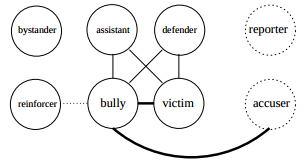
\includegraphics[width=0.3\textwidth]{bullyDiagram}	
  \caption{Graph of bullying and its relations.}
  \label{fig:bully-figure}
\end{figure}

\paragraph{Non Binary Classifier}
This project only trains a binary classifier for bullying. Unfortunately, bullying is a complex issue and has many more parts than just bullying and not bullying. Often, someone who may appear to be a bully is simply reporting that someone else is a bully. Additionally, users who are bullies often have others who support them but who they themselves are not actually bullies. For this reason it is logical to improve the classifier to include tags for supporters, victims, bullies, and reporters. An approach which was taken by a similar project was to attempt to construct a graphical bullying map with included bullies and victims and all supporting roles. The more complete that the graph was the higher the likelihood that bullying is occuring. A visual for this can be seen in Figure~\ref{fig:bully-figure}~\cite{SentiBullying}.
\paragraph{Confirmation}
One advancement that can be made for this project is to add another layer of evaluation known as confirmation. This next layer would take the list of tweets which had been tagged as bullying by the initial evaluation and run them though another algorithm. This algorithm will then search for only that particular users tweets an run those through the analyser as well. If the second analysis comes back with several more bullying tweets then we can confirm that this person is a bully. This would improve on the fact that occasionally people have a bad day and post negative things online. However, if someone is doing it all the time it gives us proof that this person is a bully.

\begin{figure}[h!]
  %486x252 pixels
  \centering
  
\includegraphics[width=0.3\textwidth]{emoji}
  \caption{The difference between emoticon and emoji.}
  \label{fig:emoji-figure} 
\end{figure}

\paragraph{Emojis}
Twitter now has support for iPhone Emojis. Emojis are similar to emoticons but they are far more expressive than simple smile and frown faces as shown in Figure~\ref{fig:emoji-figure}. They use a format similar to html symbols using a unique unicode table representing faces and actions. Having a feature which could take into account the sentiment of Emojis would be a significant improvement to this project.
\paragraph{Seed Words}
Although the list of potential bullying words that are in use for this project is large it is still static. As bullying progresses in social media so does the associated vernacular. A feature which would improve the searching algorithm is one that will identify new seed words for future searches in the tweets which have been classified as bullying.

\paragraph{Misspellings}
On the preprocessing side some one thing that might help is correcting common misspellings for words. By correcting these misspellings we may be able to find them in our lexical resources and have more features fire. A tweet is limited to 140 characters so user often shorten words and use acronyms to be able to fit their entire message. Expanding these acronyms may have a positive effect. Finally there are negating words. These words completely change the sentiment of the word or words behind them. We change sentiment values or find the opposite words to generate a more accurate sense of the tweet.

\paragraph{More Lexicons}
Finding more lexical resources to use would be a good way making more features. We did not make use of hashtags in our current implementation but hashtags can convey a lot of information. Often times a hashtag chains multiple words together. It should be possible to split these words up and calculated a sentiment score for the hashtag. For part-of-speech we took a brute force approach but clearly some patterns carry more weight. For certain patterns we could do some more analysis and provide additional data.

\section*{Acknowledgments}
We thank Alison Rose, and Uwe Meding for their contributions in annotating our data set for this project. Without their efforts this project would not have been possible.
Additionally, we would like to thank Willam Boag for providing us with lexicons from a similar project which proved to be immensely helpful.


% We need to add references to any documents used as well       
\bibliographystyle{plain}
\bibliography{References}

% example of adding references
% I switched this to use BibTex which is standard now as opposed to what they suggested. 
% In the References.bib file you can find a list of the articles. just follow the same format and look at bibtex formatting if you have any issues.

\end{document}
